\section*{Question 3: SVM}

\subsection*{a+b)}
\begin{figure}[H]
\caption{Linear SVM by inspection}
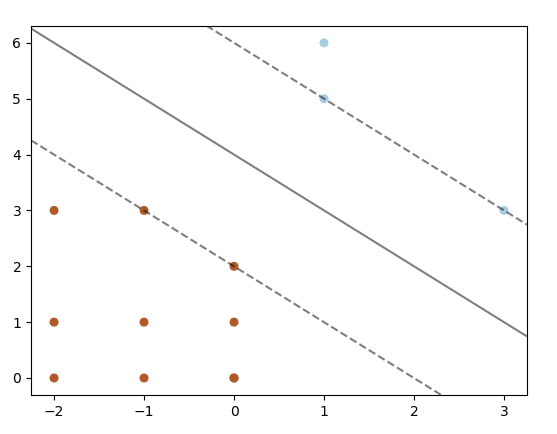
\includegraphics[width=8cm]{svm1.png}
\centering
\end{figure}

\begin{center}
Parameters $w_1$ = -0.5
$w_2$ = -0.5
b = 2

to fit the equation $w_1 x_1$ + $w_2 x_2$ + b = 0
\end{center}

\subsection*{c)}
\begin{figure}[H]
\caption{Linear SVM by inspection}
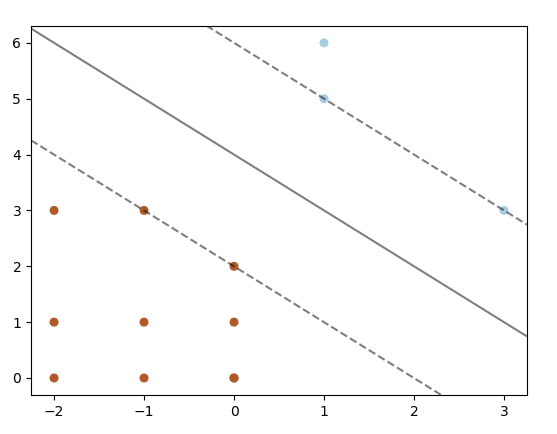
\includegraphics[width=8cm]{svm2.png}
\centering
\end{figure}

\begin{center}
Parameters $w_1$ = -0.5
$w_2$ = -0.5
b = 2

to fit the equation $w_1 x_1$ + $w_2 x_2$ + b = 0\\
\end{center}
The parameters are still the same because the new points do not change the margins, so the hyperplane stays the same.